\begin{frame}{Datenschutz}
  \centering 
  
  \note[item]{Überall werden Daten erhoben}
  \note[item]{
    Manchmal eindeutig 
    \begin{itemize}
      \item Eingabe von Daten bei Kontoerstellung
    \end{itemize}
  }
  \note[item]{
    Aber viel öfter ohne wirkliches Wissen
    \begin{itemize}
      \item Tracker auf Websites
      \item Nutzung anderer Dienste
    \end{itemize}
  }
  \note[item]{
    Deswegen Datenschutz wichtig
  }

  
\includegraphics[width=0.45\textwidth]{images/computer_data_tobu} 
\end{frame}

\begin{frame}{Datenschutz}

  \note<1->[item]{Definition aus Paper von Lee et al. (meine Zusammenfassung u. Übersetzung)}
  \note<2->[item]{Schutz vor unauthorisiertem Zugriff}
  \note<3->[item]{Sicherung, dass die Daten angemessen genutzt werden}
  \note<4->[item]{Korrektheit und Vollständigkeit gesammelter Daten über Personen}
  \note<5->[item]{Verfügbarkeit der Daten für das Subjekt und die Sicherung der Rechte des Subjekts an seinen Daten}
  \note<6->[item]{Sicherung der Rechte des Subjekts die Daten einzusehen, aktualisieren oder korrigieren}

  Nach Lee et al.\cite{lee_ethical_2016}:

  \begin{block}{Datenschutz}
    \begin{itemize}
      \item<2->{Schutz vor unauthorisiertem Zugriff}
      \item<3->{Sicherung, dass die Daten angemessen genutzt werden}
      \item<4->{Korrektheit und Vollständigkeit gesammelter Daten über Personen}
      \item<5->{Verfügbarkeit der Daten für das Subjekt und das Besitzrecht des Subjekts an seinen Daten}
      \item<6->{Sicherung der Rechte des Subjekts die Daten einzusehen, aktualisieren oder korrigieren}
    \end{itemize} 
  \end{block}
\end{frame}

\begin{frame}{Datenschutz}
  \centering

  \note<1->[item]{Selbes Paper}
  \note<1->[item]{Gesetz und Ethik sind verbunden}
  \note<2->[item]{Gesetz gibt Ethik Durchsetzungsvermögen \begin{itemize}
      \item Bsp. Ethischer Schluss: Stehlen ist falsch
      \item Aber ohne Gesetz: keine Durchsetzung
    \end{itemize}
  }
  \note<3->[item]{Ethik gibt Gesetz Kontext \begin{itemize}
      \item Bsp. Arbeit in Niedriglohnländer auszulagern ist legal, aber ist es ethisch?
    \end{itemize}
  }
  \note<3->[item]{Ethische Ideen über Datenschutz werden im Gesetz umgesetzt.}
  \note<3->[item]{Sehen das später etwas mehr}

  \begin{tikzpicture}
    \node (law) {
\includegraphics[width=0.25\textwidth]{images/book_law}};
    \node[below = 0cm of law] (law-name) {Gesetz};
    \node[right = 4cm of law] (ethics) {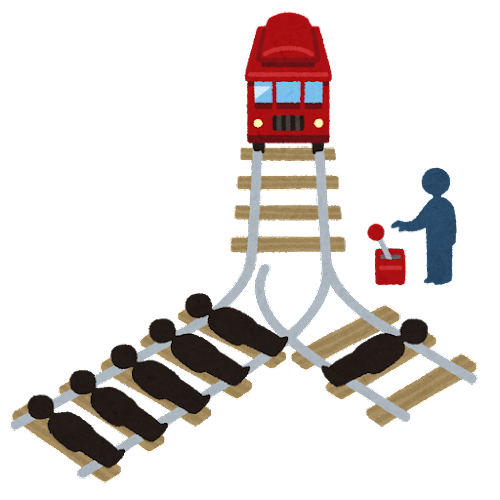
\includegraphics[width=0.25\textwidth]{images/trolley_problem}};
    \node[below = 0cm of ethics] (ethics-name) {Ethik};

    \draw<2->[-stealth] (law) to[out = 20, in = 160, edge node={node[above] {Kann durchsetzen}}] (ethics);
    \draw<3->[-stealth] (ethics) to[out = 200, in = 340, edge node={node[below] {Gibt Kontext}}] (law);
  \end{tikzpicture}

\end{frame}

